\documentclass[12pt]{article}
\usepackage[utf8]{inputenc}
\usepackage{geometry}
\usepackage{svg}
\usepackage{float}
\usepackage{caption}
\usepackage{amsmath,amsthm,amsfonts,amssymb,amscd}
\usepackage{fancyhdr}
\usepackage{titlesec}
\usepackage{hyperref}
\usepackage{listings}
\usepackage[skip=3pt]{parskip}
\usepackage[ngerman]{babel}
\pagestyle{empty}
\titleformat*{\section}{\large\bfseries}
\titleformat*{\subsection}{\bfseries}

%
\geometry{
	a4paper,
	total={170mm,240mm},
	left=20mm,
	top=30mm,
}

\date{}
%Bitte ausfüllen
\newcommand\course{Software Architectures for Enterprises}
\newcommand\hwnumber{\large Portfolio 1}
\newcommand\Name{Fabian Sponholz}
\newcommand\Neptun{1561546}

%Matheinheiten
\newcommand\m{\:\textrm{m}}
\newcommand\M{\:\Big[\textrm{m}\Big]}
\newcommand\mm{\:\textrm{mm}}
\newcommand\MM{\:\Big[\textrm{mm}\Big]}
\newcommand\un{\underline}
\newcommand\s{\:\textrm{s}}
\newcommand\bS{\:\Big[\textrm{S}\Big]}
\newcommand\ms{\:\frac{\textrm{m}}{\textrm{s}}}
\newcommand\MS{\:\Big[\frac{\textrm{m}}{\textrm{s}}\Big]}
\newcommand\mss{\:\frac{\textrm{m}}{\textrm{s}^2}}
\newcommand\MSS{\:\Big[\frac{\textrm{m}}{\textrm{s}^2}\Big]}

%Trennlinie
\newcommand\separator{\rule{\linewidth}{0.5pt}}

%Bitte nicht einstellen
\renewcommand{\figurename}{Abbildung}
\renewcommand{\tablename}{Tabelle}
\pagestyle{fancyplain}
\headheight 35pt
\lhead{\Name\\\Neptun}
\chead{\textbf{ \hwnumber}}
\rhead{\course \\ \today}
\lfoot{}
\cfoot{}
\rfoot{\small\thepage}
\headsep 1.5em

\begin{document}
	
\section*{Aufgabe 1 - Thread-Basierte Glühwürmchen}
Zunächst wollte ich die Aufgabe um der alten Traditionen Willen in JavaScript lösen, leider ist mir dabei aber klar geworden, dass Multithreading und JavaScript noch schlechter zusammen passen als OpenCL und JavaScript.

Schlussendlich habe ich mich also dazu entschieden, die Aufgabe in Java zu realisieren, da es hier eine sehr komfortable Implementierung von Mutli-Threading gibt, und außerdem einige sehr ausgereifte UI-Bibliotheken.

Meine Implementierung besteht aus drei Klassen und einem Interface:
\begin{enumerate}
	\item \texttt{class Main} JavaFX-Oberfläche, die die Glühwürmchen-Threads initialisiert und visualisiert.
	\item \texttt{class Firefly} Implementiert \texttt{Runnable} und repräsentiert somit die Glühwürmchen-Threads. Sie erbt außerdem von \texttt{Rectangle} und kann sich somit direkt selbst in JavaFX visualisieren.
	\item \texttt{class TorusTopology} Helfer-Klasse, die aus einem gegebenen 2-dimensionalen Array von Objekten die Nachbarn eines gegebenen Objektes in einem Torus zurückgibt.
	\item \texttt{interface Topology} Interface, das die \texttt{getNeighbours()}-Methode enthält. Das Interface wird von der \texttt{TorusTopology}-Klasse implementiert und ist vorhanden, um einfacher weitere Topologien implementieren zu können.
\end{enumerate}

Die Synchronisation der Glühwürmchen funktioniert nachrichtenbasiert: Immer wenn ein Glüh-würmchen seine Phase von leuchtend auf nicht leuchtend oder umgekehrt wechselt, wird auf allen benachbarten Glühwürmchen die Methode \texttt{iAmFlashing(boolean isFlashing)} aufgerufen. Falls der Phasen-Zustand der beiden Glühwürmchen nicht übereinstimmt, wird die Phase des entsprechenden benachbarten Glühwürmchens um einen bestimmten Wert (\texttt{double coupling}) verschoben.

Die Main-Klasse erstellt ein Feld aus MxN Glührürmchen und visualisiert diese in einem JavaFX-Fenster. Dann werden mithilfe der \texttt{TorusTopology}-Klasse die Nachbarn jedes Glüh-würmchens ermittelt und entsprechend in den \texttt{Firefly}-Objekten gesetzt.

\subsection*{Aufruf des Programms}
Zum Bauen des Programms wurde das Build-Tool \emph{Gradle} verwendet. Dieses muss nicht erst installiert werden, sondern kann direkt mithilfe des Gradle-Wrappers (\texttt{./gradlew} bzw für Windows \texttt{./gradlew.bat}) aufgerufen werden.

Folgender Befehl baut und startet das Programm:

\texttt{./gradlew run}

\begin{figure}[H]
	\centering
	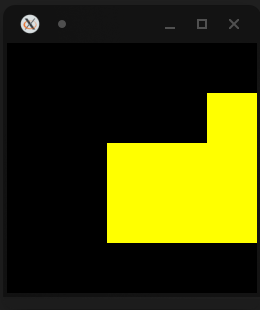
\includegraphics[width=0.5\textwidth]{./img/screenshot_threading}
	\caption{GUI der Threading-Implementierung}
\end{figure}

\subsection*{Besondere Vorkommnisse}
Bei der Implementierung der Threading-Variante bin ich auf keine besonderen Schwierigkeiten gestoßen. Nachdem ich einmal verstanden habe, dass man den Algorithmus auch auf diese Weise (durch Benachrichtigung der Nachbarn beim Phasenwechsel) realisieren kann, war die Implementierung recht einfach.

\section*{Aufgabe 2 - Jedes Glühwürmchen ein Prozess (IPC / gRPC)}
Deutlich komplexer wurde die Implementierung der Glühwürmchen mit Inter-Prozess-Kommunikation anstatt Multithreading. Hier mussten nicht nur zwei unabhängige Programme geschrieben werden (eines simuliert das Glühwürmchen, eines dient der Beobachtung), sondern es mussten noch einige zusätzliche Hürden überwunden werden:

\begin{itemize}
	\item Kommunikation untereinander mit gRPC
	\item Dynamische Visualisierung der vorhandenen Glühwürmchen.
	\item Geordnetes Starten von Glühwürmchen-Prozessen, sodass diese einen Torus repräsentieren
\end{itemize}

Im Folgenden werde ich erklären, wie ich diese Hürden überwunden habe.

\subsection*{Kommunikation zwischen den Glühwürmchen}
Für die Kommunikation untereinander habe ich mich für das Remote-Procedure-Call-Protokoll \emph{gRPC} entschieden. Dieses ermöglicht den Aufruf von Methoden in Java-Programmen, die in anderen Prozessen oder gar auf anderen Maschinen laufen, da es auf dem TCP-Protokoll aufbaut.

Dadurch steht fest, dass jedes Glühwürmchen auf einem anderen Port auf die Anfragen anderer Glühwürmchen lauschen muss. Somit kann jedes Glühwürmchen eindeutig durch seine Server-Portnummer identifiziert werden. Bei der Initialisierung wird einem Glühwürmchen über Kommandozeilen-Argumente zuerst die eigene Port-Nummer übergeben, und dann alle Portnummern der Nachbar-Glühwürmchen.

Zur Kommunikation muss zunächst ein Prototyp-File erstellt werden, in dem die verfügbaren Methoden sowie Parameter- und Return-Typen definiert sind. Diese befindet sich im Verzeichnis \texttt{./src/main/proto} und dort wird eine Methode \texttt{notifyFirefly} mit Parameter-Typ \texttt{FireflyRequest} und Return-Typ \texttt{FireflyReply} definiert.
Der \texttt{FireflyRequest} enthält die wichtigen Informationen: 
\begin{itemize}
	\item \texttt{bool isFlashing} zeigt an, ob das sendende Glühwürmchen gerade leuchtet oder nicht.
	\item \texttt{int32 port} enthält die Information, welchen Server-Port das sendende Glühwürmchen hat. Dadurch kann es vom Firefly-Observer identifiziert und dargestellt werden.
\end{itemize}

Der Return-Typ ist im Grunde irrelevant, muss aber definiert werden.

Die Kommunikation über gRPC habe ich in die Klassen \texttt{FireflyServer} und \texttt{FireflyClient} gekapselt, um davon zu abstrahieren und mich nirgendwo sonst mit den Eigenheiten von gRPC herumschlagen zu müssen. Die Klasse \texttt{FireflyServer} bekommt abgesehen von einem Port auch ein Objekt vom Typ \texttt{FireflyCallable} übergeben, welches eine Methode \texttt{flashStatusChanged()} enthält, die aufgerufen wird, wenn der Server einen Methodenaufruf empfängt.

Der \texttt{FireflyClient} bekommt einen Port übergeben, der den Server identifiziert, an den dieser Client senden soll. Außerdem stellt er eine Methode \texttt{notifyFirefly()} bereit, über die der entsprechende Server angefragt wird.

Jedes Glühwürmchen hat also einen \texttt{FireflyServer}, über den andere Glühwürmchen es erreichen können, und eine Anzahl $n > 0$ an \texttt{FireflyClients}, die die Nachbarn des Glühwürmchens repräsentieren. Die restliche Logik konnte weitestgehend aus Aufgabe 1 übernommen werden.

\subsection*{Visualisierung der Glühwürmchen}

\subsection*{Generierung und Visualisierung eines Torus}
	
\end{document}